\section{\(\epsilon\)-Non-deterministic Finite Automata}
\par Recall that the set of all strings over \(\Sigma\) is defined as
the type \(List\ \Sigma^*\). However, this definition gives us no way to
extract an \(\epsilon\) alphabet from the input string. Therefore,
we need to introduce another representation specific to this
purpose. The representation in defined under the module
\textbf{\(\Sigma\)-with-\(\epsilon\)} in \textbf{Language.agda} along
with itis related operations and lemmas. 

\begin{defn}
\noindent We define \(\Sigma^e\) as the union of
\(\Sigma\) and \(\{\epsilon\}\), i.e. \(\Sigma^e = \Sigma \cup \{\epsilon\}\).
\end{defn} 

\par The equivalent data type is as follow:
\begin{lstlisting}[mathescape=true,xleftmargin=.3\textwidth]
data $\Sigma^e$ : Set where
  $\alpha$ : $\Sigma \to \Sigma^e$
  E : $\Sigma^e$
\end{lstlisting}

\par All the alphabets in \(\Sigma\) are included in \(\Sigma^e\) by using the
\(\alpha\) constructor while the \(\epsilon\) alphabet corresponds to
the constructor \(E\) in the data type. 

\begin{defn}
\noindent Now we define \(\Sigma^{e*}\), the set of all strings over
\(\Sigma^e\) in a way similar to \(\Sigma^*\), i.e. \(\Sigma^{e*} =
List\ \Sigma^e\). 
\end{defn}

\par For example, the string 'Agda' can be
represented by (\(\alpha\ A :: \alpha\ g :: E :: \alpha\ d :: E :: \alpha\
a :: [\ ]\)) or (\(E :: \alpha\ A :: E :: E :: \alpha\ g :: \alpha\ d ::
E :: \alpha\ a :: [\ ]\)). We call these two lists as the \(\epsilon\)-strings of the
string 'Agda'. 

\begin{defn}
\noindent Now we define \(to\Sigma^*(w^e)\) as a function that takes an
\(\epsilon\)-string of \(w\), \(w^e\) and returns \(w\). 
\end{defn}

\par It is define in Agda as follow: 
\begin{lstlisting}[mathescape=true,xleftmargin=.3\textwidth]
to$\Sigma^*$ : $\Sigma^{e*}$ $\to$ $\Sigma^*$
to$\Sigma^*$ [] = []
to$\Sigma^*$ ($\alpha$ a :: w) = a :: to$\Sigma^*$ w
to$\Sigma^*$ (E :: w) = to$\Sigma^*$ w
\end{lstlisting}

\par Now, let us define \(\epsilon\)-NFA using \(\Sigma^{e*}\). The
type of \(\epsilon\)-NFA is defined in \textbf{eNFA.agda} along with its operations and
properties. 

\begin{defn}
\noindent An \(\epsilon\)-NFA is a 5-tuple \(M = (Q
,\ \Sigma^e,\ \delta,\ q_0,\ F)\), where
\begin{enumerate}[nolistsep]
  \item \(Q\) is a finite set of states;
  \item \(\Sigma^e\) is the union of \(\Sigma\) and \(\{\epsilon\}\);
  \item \(\delta\) is a mapping from \(Q \times \Sigma^e\) to
    \(\mathcal P \left({Q}\right)\) that defines the behaviour of the automata;
  \item \(q_0\) in \(Q\) is the initial state;
  \item \(F \subseteq Q\) is the set of accepting states. 
\end{enumerate}
\end{defn}

\par It is formalised as a record in Agda as shown below: 

\begin{lstlisting}[mathescape=true,xleftmargin=.3\textwidth]
record $\epsilon \hyphen$NFA : Set$_1$ where
  field
    Q      : Set
    $\delta$       : Q $\to$ $\Sigma^e$ $\to$ DecSubset Q
    q$_0$      : Q
    F      : DecSubset Q
    $\forall$qEq    : $\forall$ q $\to$ q $\in^d$ $\delta$ q E
    Q?     : DecEq Q
    |Q|-1  : $\mathbb{N}$
    It     : Vec Q (suc |Q|-1)
    $\forall$q$\in$It    : (q : Q) $\to$ (q $\in^V$ It)
    unique : Unique It
\end{lstlisting}

\par The set of alphabets \(\Sigma\) is passed into the module as a
parameter and \(\Sigma^e\) is constructed using \(\Sigma\). Together with \(Q\), \(\delta\),
\(q_0\) and \(F\), these five fields correspond to the 5-tuple
\(\epsilon\)-NFA. The other extra fields are used when computing
\(\epsilon\)-closures. They are \(\forall qEq\) -- a proof that any
state in \(Q\) can reach itself by an
\(\epsilon\)-transition; \(Q?\) -- the decidable equality of \(Q\);
\(|Q|-1\) -- the number of states minus 1; \(It\) -- a vector
containing all the states in \(Q\); \(\forall q\in It\)
-- a proof that every state in \(Q\) is also in the vector
\(It\); and \(unique\) -- a proof that there is no repeating elements in
\(It\). 

\par Now, before we can define the accepting language of a given
\(\epsilon\)-NFA, we need to define several operations of
\(\epsilon\)-NFA. 

\begin{defn}
\noindent A configuration is composed of a state and an alphabet from
\(\Sigma^e\), i.e. \(C = Q \times \Sigma^e\). 
\end{defn}

\begin{defn}
\noindent A move in an \(\epsilon\)-NFA is
represented by a binary function (\(\vdash\)) on two configurations. We say
that for all \(w \in \Sigma^{e*}\) and \(a \in \Sigma^e\), \((q, aw)
\vdash (q' , w)\) if and only if \(q' \in \delta (q , a)\). 
\end{defn}

\par The binary function is defined in Agda as follow: 
\begin{lstlisting}[mathescape=true,xleftmargin=.3\textwidth]
  _$\vdash$_ : (Q $\times$ $\Sigma^e$ $\times$ $\Sigma^{e*}$) $\to$ (Q $\times$ $\Sigma^{e*}$) $\to$ Set
  (q , a , w) $\vdash$ (q' , w') = w $\equiv$ w' $\times$ q' $\in^d$ $\delta$ q a
\end{lstlisting}

\begin{defn}
\noindent Suppose \(C\) and \(C'\) are two configurations. We say that \(C \vdash^0 C'\) if and only
if \(C = C'\); and \(C_0 \vdash^k C_k\) for any \(k \geq 1\) if and only if there exists a chain of
configurations \(C_1, C_2, ..., C_{k-1}\) such that \(C_i \vdash C_{i+1}\) for all \(0 \leq i < k\). 
\end{defn}

\par It is defined as a recursive function in Agda as follow: 
\begin{lstlisting}[mathescape=true,xleftmargin=.3\textwidth]
  _$\vdash^k$_-_ : (Q $\times$ $\Sigma^{e*}$) $\to$ $\mathbb{N}$ $\to$ (Q $\times$ $\Sigma^{e*}$) $\to$ Set
  (q , w$^e$) $\vdash^k$ zero  - (q' , w$^e$')
    = q $\equiv$ q' $\times$ w$^e$ $\equiv$ w$^e$'
  (q , w$^e$) $\vdash^k$ suc n - (q' , w$^e$') 
    = $\exists$[ p $\in$ Q ] $\exists$[ a$^e$ $\in$ $\Sigma^e$ ] $\exists$[ u$^e$ $\in$ $\Sigma^{e*}$ ]
      (w$^e$ $\equiv$ a$^e$ :: u$^e$ $\times$ (q , a$^e$ , u$^e$) $\vdash$ (p , u$^e$) $\times$ (p , u$^e$) $\vdash^k$ n - (q' , w$^e$'))
\end{lstlisting}

\begin{defn}
\noindent We say that \(C \vdash^* C'\) if and only
if there exists a number of chains \(n\) such that \(C \vdash^n C'\). 
\end{defn}

\par Its corresponding type is defined as follow: 
\begin{lstlisting}[mathescape=true,xleftmargin=.3\textwidth]
  _$\vdash^*$_ : (Q $\times$ $\Sigma^{e*}$) $\to$ (Q $\times$ $\Sigma^{e*}$) $\to$ Set
  (q , w$^e$) $\vdash^*$ (q' , w$^e$') = $\exists$[ n $\in$ $\mathbb{N}$ ] (q , w$^e$) $\vdash^k$ n - (q' , w$^e$')
\end{lstlisting}

\begin{defn}
\label{defn:enfa}
\noindent For any string \(w\), it is accepted by an \(\epsilon\)-NFA
if and only if there exists an \(\epsilon\)-string of \(w\)
that can take \(q_0\) to an accepting state \(q\). Therefore, the
accepting language of an \(\epsilon\)-NFA is given by the set \(\{w\ |\ \exists w^e\in
\Sigma^{e*}.\ w = to\Sigma^*(w^e) \wedge \exists q\in F.\ (q_0,w^e) \vdash^* (q,\epsilon)\}\). 
\end{defn}

\par The corresponding formalisation in Agda is as follow: 
\begin{lstlisting}[mathescape=true,xleftmargin=.3\textwidth]
  L$^{eN}$ : $\epsilon \hyphen$NFA $\to$ Language
  L$^{eN}$ nfa = $\lambda$ w $\to$ 
            $\exists$[ w$^e$ $\in$ $\Sigma^{e*}$ ] (w $\equiv$ $to\Sigma^*$ w$^e$ $\times$ ($\exists$[ q $\in$ Q ] (q $\in^d$ F $\times$ (q$_0$ , w$^e$) $\vdash^*$ (q , []))))
\end{lstlisting}

\section{Thompson's Construction}
\par Now, let us look at the translation of regular expressions to
\(\epsilon\)-NFA. The translation is defined as the function
\textbf{regexToeNFA} in \textbf{Translation/RegExp-eNFA.agda} while
the constructions of states are defined in \textbf{State.agda}. 

\begin{defn}
\label{defn:thompson}
\noindent The translation of regular expressions
to \(\epsilon\)-NFA is defined inductively as follow:
\begin{enumerate}[nolistsep]
  \item for \(\O\), we have \(M = (\{init\},\ \Sigma^e,\ \delta,\
    init,\ \O)\) and graphically, \begin{center}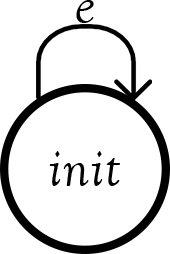
\includegraphics{null}\end{center}
  \item for \(\epsilon\), we have \(M = (\{init\},\ \Sigma^e,\
    \delta,\ init,\ \{init\})\) and graphically, \begin{center}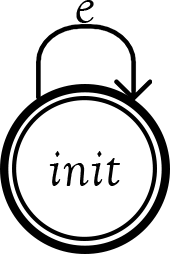
\includegraphics{epsilon}\end{center}
  \item for \(a\), we have \(M = (\{init, accept\},\ \Sigma^e,\
    \delta,\ init,\ \{accept\})\) and graphically, \begin{center}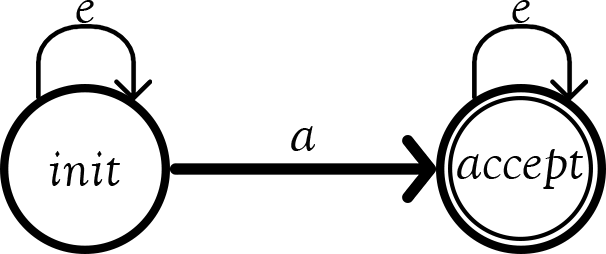
\includegraphics{singleton}\end{center}
  \item suppose \(N_1 = (Q_1,\ \delta_1,\ q_{01},\ F_1)\) and \(N_2 =
    (Q_2,\ \delta_2,\ q_{02},\ F_2)\) are \(\epsilon\)-NFAs translated from the
    regular expressions \(e_1\) and \(e_2\) respectively, then
    \begin{enumerate}[nolistsep]
      \item for \((e_1\ |\ e_2)\), we have \(M = (\{init\} \cup Q_1
        \cup Q_2,\ \Sigma^e,\ \delta,\ init,\ F_1 \cup F_2)\) and
        graphically, \begin{center}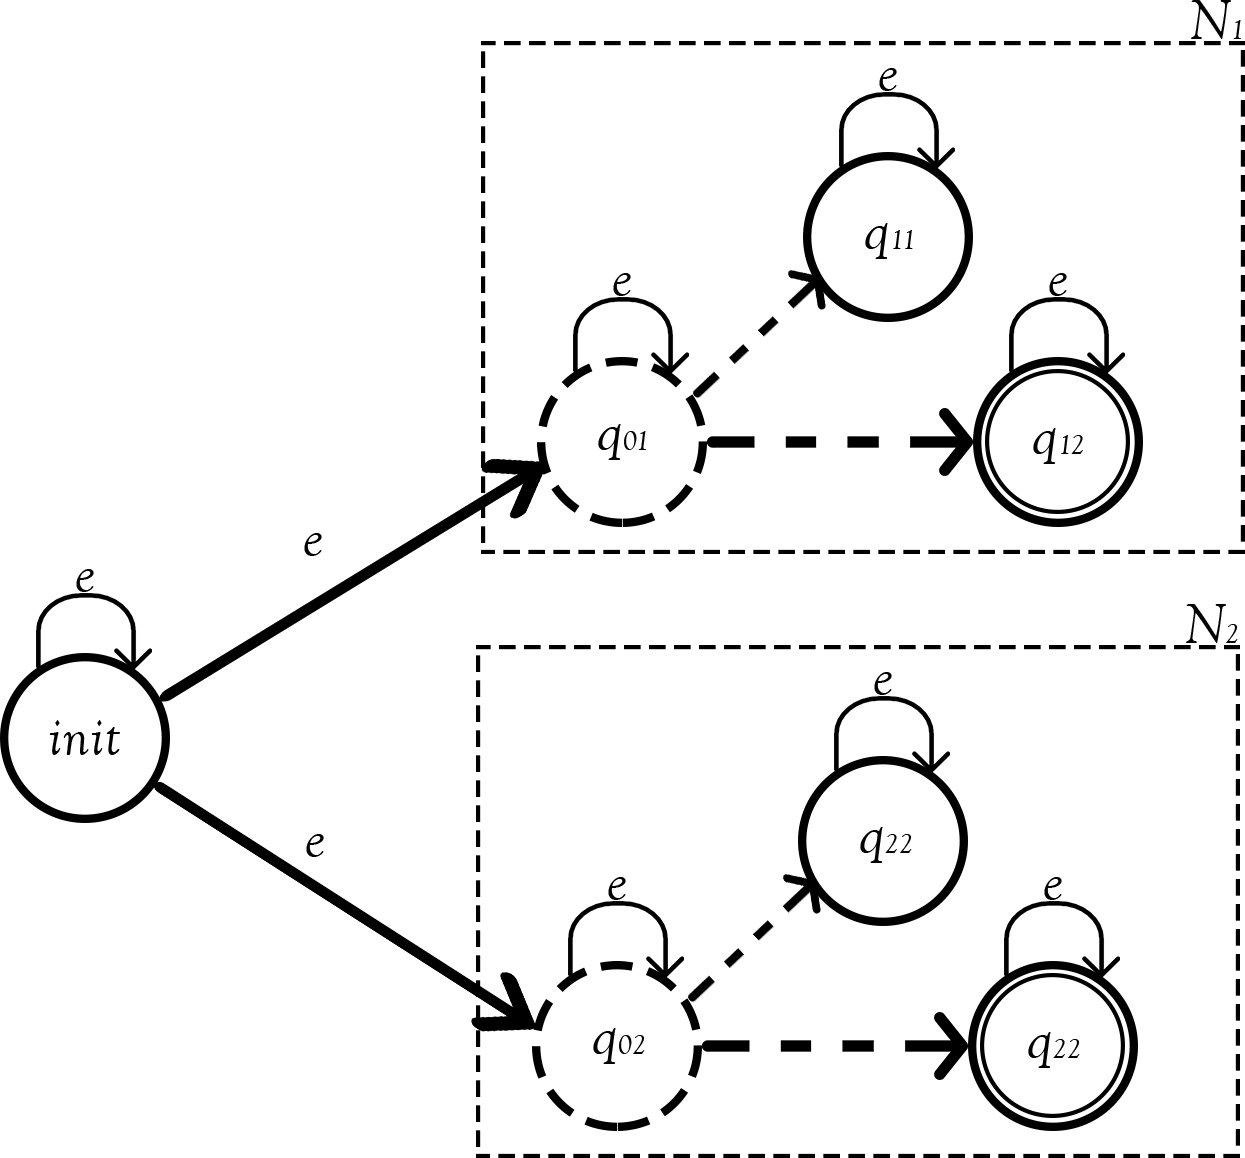
\includegraphics{union}\end{center}
      \item for \(e_1\cdot e_2\), we have \(M = (Q_1 \cup \{mid\}
        \cup Q_2,\ \Sigma^e,\ \delta,\ init,\ F_2)\) and graphically, \begin{center}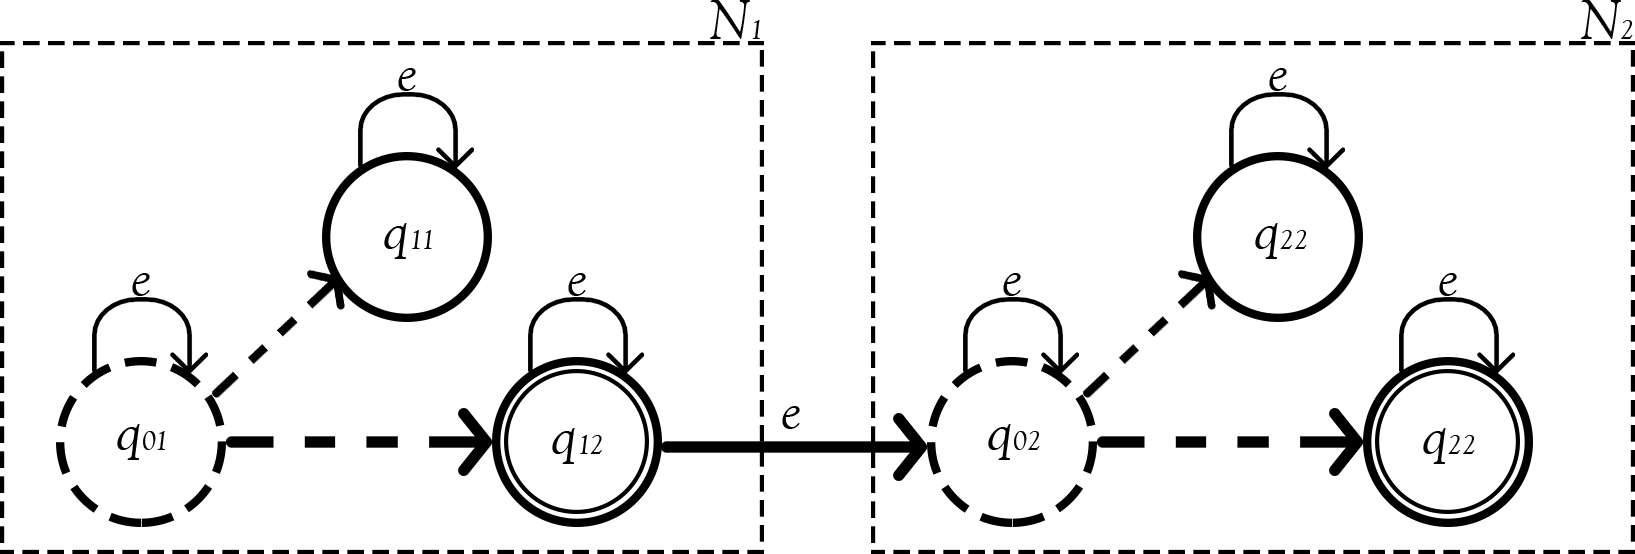
\includegraphics{concat}\end{center}
      \item for \(e_1^{\ *}\), we have \(M = (\{init\} \cup Q_1,\
        \Sigma^e,\ \delta,\ init,\ \{init\} \cup F_1)\) and
        graphically, \begin{center}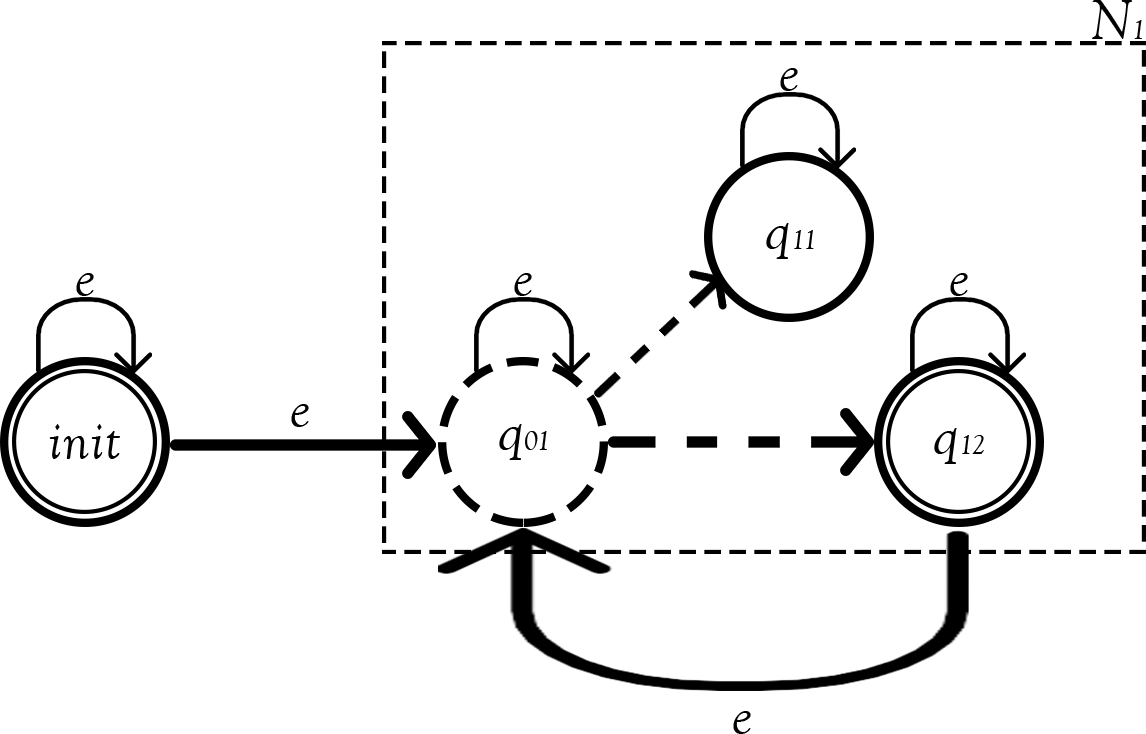
\includegraphics{star}\end{center}
     \end{enumerate}
\end{enumerate}
\end{defn}

\par Apart from the five fields, the other fields in the record
\textit{\(\epsilon\)-NFA} are also constructed by the function. Now, let us prove the correctness of the above translation by
proving that their accepting languages are equal. The correctness
proof is defined as the function \mmb{L^R \!\approx\! L^{eN}} in
\textbf{Correctness.agda} while the detail proofs are
defined in \textbf{Correctness/RegExp-eNFA.agda}. 

\begin{thm} 
\noindent For any given regular expression, \(e\), its accepting
language is equal to the language accepted by the \(\epsilon\)-NFA
translated from \(e\) using Thompson's Construction, i.e. \(L(e) =
L(\)translated \(\epsilon\)-NFA\()\). 
\end{thm} 

\begin{proof}
\noindent We can prove the theorem by induction on regular
expressions. 

\par \noindent \textbf{Base cases.}\quad By \autoref{defn:thompson}, it is
obvious that the statement holds for \(\O\), \(\epsilon\) and
\(a\). 

\par \noindent \textbf{Induction hypothesis 1.}\quad For any two regular expressions
\(e_1\) and \(e_2\), let \(N_1 =
(Q_1,\ \delta_1,\ q_{01},\ F_1)\) and \(N_2 = (Q_2,\ \delta_2,\
q_{02},\ F_2)\) be their translated \(\epsilon\)-NFA 
respectively, we assume that \(L(e_1) = L(N_1)\) and \(L(e_2) =
L(N_2)\). 

\par \noindent \textbf{Inductive steps.}\quad There are three cases: 1)
\(e_1\ |\ e_2\), 2) \(e_1 \cdot e_2\) and 3) \(e_1^{\ *}\). 

\par \noindent 1) \textit{Case \((e_1\ |\ e_2)\)}:\quad Let \(M = (Q,\ \delta,\ q_0,\ F) = (\{init\} \cup Q_1 \cup Q_2,\
\delta,\ init,\ F_1 \cup F_2)\) be its translated \(\epsilon\)-NFA. Then for any string \(w\), 

\par 1.1) if \((e_1\ |\ e_2)\) accepts \(w\), then by
\autoref{defn:regex} and \autoref{defn:lang_union},
either i) \(e_1\) accepts \(w\) or ii) \(e_2\) accepts \(w\). Assuming case i), then by
induction hypothesis, \(N_1\) also accepts \(w\). Therefore, there
must exist an \(\epsilon\)-string of \(w\), \(w^e\), that can take \(q_{01}\)
to an accepting state \(q\) in \(N_1\). Now, consider another
\(\epsilon\)-string of \(w\), \(\epsilon w^e\), it can
take \(init\) to \(q\) in \(M\) because \(\epsilon\) can take \(init\)
to \(q_{01}\). Recall that \(q\) is an accepting
state in \(N_1\); therefore, \(q\) is also an accepting state in
\(M\) and thus, by \autoref{defn:enfa}, \(M\) accepts \(w\). The same argument also applies
to the case when \(e_2\) accepts \(w\); therefore, \(L(e_1\ |\ e_2) \subseteq L(M)\) is true; 

\par 1.2) if \(M\) accepts \(w\), then by \autoref{defn:enfa}, there must exist an
\(\epsilon\)-string of \(w\), \(w^e\), that can take \(init\) to an
accepting state \(q\) in \(M\). \(q\) must be different from \(init\) because
\(q\) is an accepting state but \(init\) is not. Now, by
\autoref{defn:thompson}, there are only two possible ways for \(init\) to reach \(q\) in \(M\), i)
via \(q_{01}\) or ii) via \(q_{02}\). Assuming case i), then \(w^e\)
must be in the form of \(aw'^e\) because \(\epsilon\) is the only alphabet that can take
\(init\) to \(q_{01}\) and thus \(w'^e\) can take \(q_{01}\) to \(q\). Furthermore, \(q\) is an
accepting state in \(M\); therefore, \(q\) is also an accepting
state in \(N_1\) and thus \(N_1\) accepts \(w\). By induction hypothesis, \(e_1\) also accepts \(w\);
therefore, we have \(w \in L(e_1\ |\ e_2)\). The same argument also
applies to case ii) and thus \(L(e_1\ |\ e_2) \supseteq L(M)\) is true; 

\par 1.3) combining 1.1 and 1.2, we have \(L(e_1\ |\ e_2) = L(M)\). 

\par \noindent 2) \textit{Case \((e_1 \cdot e_2)\)}:\quad Let \(M = (Q,\
\delta,\ q_0,\ F) = (Q_1 \cup \{mid\} \cup Q_2,\ \delta,\ q_{01},\
F_2)\) be its translated \(\epsilon\)-NFA. Then for any string
\(w\), 

\par 2.1) if \((e_1 \cdot e_2)\) accepts \(w\), then by
\autoref{defn:regex} and \autoref{defn:lang_con}, there must exist a string \(u \in L(e_1)\) and a string \(v \in L(e_2)\) such that \(w
= uv\). By induction hypothesis, \(N_1\) accepts \(u\) and \(N_2\)
accepts \(v\). Therefore, there must exist i) an \(\epsilon\)-string
of \(u\), \(u^e\), that can take \(q_{01}\) to an accepting state \(q_1\) in
\(N_1\) and ii) an \(\epsilon\)-string of \(v\), \(v^e\), that can take
\(q_{02}\) to an accepting state \(q_2\) in \(N_2\). Now, let us
consider another \(\epsilon\)-string of \(w\), \(u^e\epsilon \epsilon
v^e\), it can take \(q_{01}\) to \(q_2\) in \(M\) because \(u^e\) takes
\(q_{01}\) to \(q_1\), \(\epsilon\) takes \(q_1\) to \(mid\), another
\(\epsilon\) takes \(mid\) to \(q_{02}\) and \(v^e\) takes \(q_{02}\)
to \(q_2\). Furthermore, \(q_2\)
is also an accepting state in \(M\) because \(q_2\) is an accepting
state in \(N_2\). Therefore, \(M\) accepts \(w\)
and thus \(L(e_1 \cdot e_2) \subseteq L(M)\) is true; 

\par 2.2) if \(M\) accepts \(w\), then by \autoref{defn:enfa}, there must
exist an \(\epsilon\)-string of \(w\), \(w^e\), which can take
\(q_{01}\) to an accepting state \(q\) in \(M\). Since \(q\) is an
accepting state in \(M\); therefore, \(q\) must be in \(Q_2\). The only possible way for
\(q_{01}\) to reach \(q\) is by going through the state \(mid\). Therefore, there must exist i) an \(\epsilon\)-string, \(u^e\), that can take
\(q_{01}\) to an accepting state \(q_1\) in \(N_1\) and ii) an
\(\epsilon\)-string \(v^e\) that can take \(q_{02}\) to \(q_2\) in
\(N_1\) and \(w^e = u^e\epsilon\epsilon v^e\). Let \(u\) and \(v\) be the normal strings of \(u^e\) and
\(v^e\) respectively, then we have \(u \in L(N_1)\), \(v \in L(N_2)\) and \(w = uv\). Now, by induction
hypothesis, \(e_1\) accepts \(u\) and \(e_2\) accepts \(v\); and thus
\(e_1 \cdot e_2\) accepts \(w\). Therefore \(L(e_1 \cdot e_2) \supseteq L(M)\) is true; 

\par 2.3) combining 2.1 and 2.2, we have \(L(e_1 \cdot e_2) = L(M)\). 

\par \noindent 3) \textit{Case \(e_1^{\ *}\)}:\quad Let \(M = (Q,\ \delta,\ q_0,\
F) = (Q_1 \cup \{mid\} \cup Q_2,\ \delta,\ q_{01},\ F_2)\) be its
translated \(\epsilon\)-NFA. Then for any string \(w\), 

\par 3.1) if \((e_1^{\ *})\) accepts \(w\), then by \autoref{defn:regex}
and \autoref{defn:lang_star}, there must exist a number \(n\) such
that \(w \in L(e_1)^n\). Now, let us do induction on \(n\). 

\par \quad \textbf{Base case.} \quad When \(n = 0\), then the language
\(L^0\) can only accept the empty string \(\epsilon\); and thus \(w =
\epsilon\). From \autoref{defn:thompson}, it is obvious that \(M\)
accepts \(\epsilon\). 

\par \quad \textbf{Induction hypothesis 2.} \quad Suppose there exists a number \(k\) such that \(w
\in L(e_1)^k\), then \(w\) is also accepted by \(M\). 

\par \quad \textbf{Induction steps.} \quad When \(n = k + 1\), by
\autoref{defn:lang_con} and \autoref{defn:lang_power}, there must
exist a string \(u \in L(e_1)\) and a string \(v \in L(e_1)^k\) such
that \(w=uv\). By induction hypothesis (1), we have \(N_1\) accepts \(u\). Therefore there must exist an \(\epsilon\)-string
\(u\), \(u^e\), that can take \(q_{01}\) to an accepting state \(q\)
in \(N_1\). Since \(q\) is an accepting state; an \(\epsilon\)
alphabet can take \(q\) back to \(q_{01}\). Furthermore, by induction
hypothesis (2), \(M\) also accepts \(v\) which implies that there
exists an \(\epsilon\)-string of \(v\), \(v^e\), that can take
\(init\) to an accepting state \(p\). Since the only
alphabet that can take \(init\) to \(q_{01}\) is \(\epsilon\); therefore,
\(v^e\) must be in the form of \(\epsilon v'^e\). Now, we have proved
that there exists an \(\epsilon\) string of \(w\), \(\epsilon u^e\epsilon v'^e\), that can
take \(init\) to an accepting state \(p\) in \(M\); and thus \(M\)
accepts \(w\). Therefore \(L(e_1^{\ *}) \subseteq L(M)\) is true; 

\par 3.2) if \(M\) accepts \(w\), then by \autoref{defn:enfa}, there must exist an
\(\epsilon\)-string \(w\), \(w^e\), that can take \(init\) to an accepting
state \(q\) with \(n\) transitions in \(M\).  If \(init = q\), then \(w\) must be an empty
string. By \autoref{defn:thompson}, it is obvious that
the empty string is accepted by \(e_1^{\ *}\). If \(init \neq q\),
then there are only two possible ways for \(init\)
to reach \(q\): 1) from \(init\) to \(q\) without going back to
\(q_{01}\) from an accepting state with an \(\epsilon\), we say that this path has no loops and 2) from \(init\)
to \(q\) with at least one loop. 
\par \quad \textit{Case 1}:\quad Since \(q \neq init\), then \(w^e\) must
be in the form of \(\epsilon w'^e\). Recall that the path has no loops, it is
obvious that \(N_1\) accepts \(w\). Therefore by
induction hypothesis (1), \(e_1\) accepts \(w\) and thus \(e_1^{\ *}\)
also accepts \(w\). 
\par \quad \textit{Case 2}:\quad Since \(q \neq init\), then \(w^e\) must
be in the form of \(\epsilon w'^e\). Recall that the path has loops, we
can separate \(w'^e\) into two parts: 1) an \(\epsilon\)-string
\(u^e\) that takes \(init\) to an accepting state \(p\) without loops
and 2) an \(\epsilon\)-string \(\epsilon v^e\) that takes \(p\) to
\(q_{01}\) to \(q\) with loops. Let \(u\) and \(v\) be the normal
string of \(u^e\) and \(\epsilon v^e\) respectively, then it is obvious that
\(w = uv\). By \textit{case 1}, \(e_1\) accepts \(u\). Now, consider
the path from \(q_{01}\) to \(q\). The path must have less than \(n\)
transitions; therefore, we can prove by induction the there must exist a number \(k\) such that
\(L(e_1)^k\) accepts \(v\). Combining the above proofs, we have \(w \in
L(e_1^{\ *})\). 
\par \quad Combining \textit{Case 1} and \textit{Case 2}, we have \(w \in L(e_1^{\ *}) \supseteq L(M)\); 

\par 3.3) combining 3.1 and 3.2, we have \(L(e_1^{\ *}) = L(M)\). 

\par \noindent Therefore, by induction, \(L(e) = L(\)translated
\(\epsilon\)-NFA\()\) is true for all any regular expression \(e\). 
\end{proof}

\newpage 
\par Below is a code snippet of our formalisation of \(L^R \subseteq
L^{eN}\). 

\begin{center} 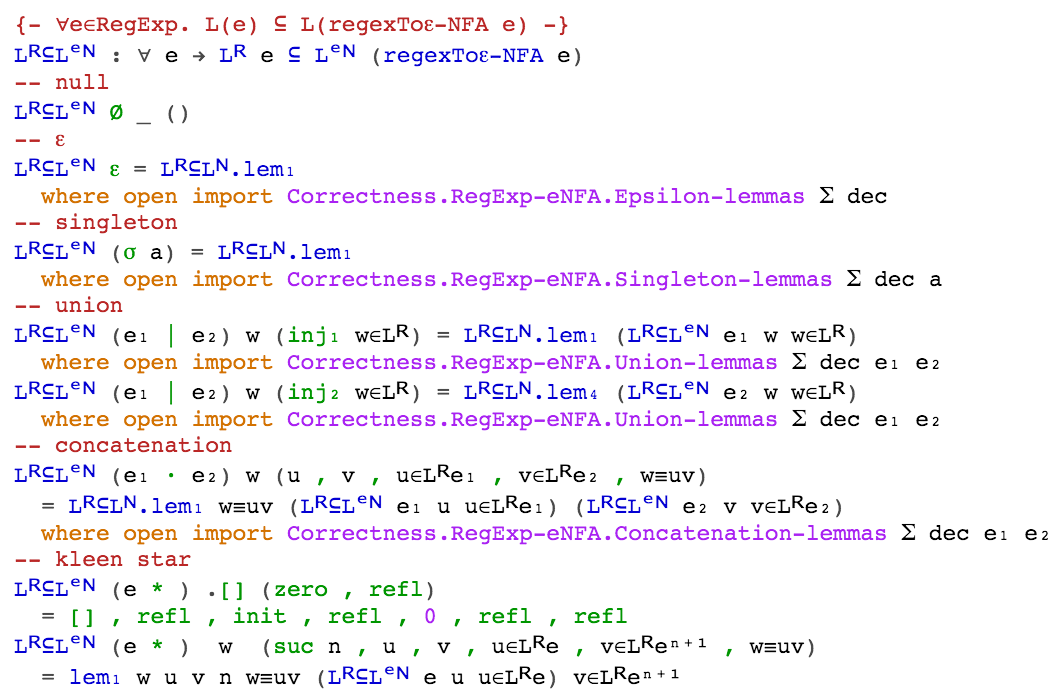
\includegraphics[width=\textwidth]{thm11} \end{center}

\par Pattern matching the regular expression corresponds to the case
analysis in the proof. As shown above, there are six cases:
\(\emptyset\), \(epsilon\), \(\sigma\ a\), union, concatenation and
kleen star. The first three correpsonds to the three base
cases. Notice that the recursive calls in last three cases is equivalent to the induction hypothesis of the
proof. These cases are equivalent to the induction steps. 